% =====================================================================
%  EE4C12 - Machine Learning for EE Applications
%  Final Project Report -- WICOS track
%  Radar & AI for Human Computer Interaction via Hand Gestures (DopNet)
%
%  HARD RULES (report is INADMISSIBLE -> FAIL if violated):
%   - English must be understandable (no typo-ridden text).
%   - At least one tested model MUST be a deep neural network (Lecture 5).
%   - All figures must be legible.
%   - Report MUST follow the proposed structure (sections below).
%  Other rules:
%   - Max 10 pages (assumed: front page + references excluded -- the
%     assignment does not state this; confirm with lecturer/TA). One report per pair. Submit as PDF + Python code
%     on Brightspace before the Week 8 deadline (late = grade 0).
%   - Do not paste full code; explain the implementation and reason about
%     the results. Short key code snippets are acceptable.
%   - TAs will run (parts of) the code and check it reproduces reported
%     results -> make sure every number/figure in here is reproducible.
%   - Good English / good code give NO extra points.
%
%  Grading rubric weights (map each to a place in the report):
%   Data analysis & pre-processing ............ 10%  -> Sec. Task 1
%   Feature selection ......................... 15%  -> Sec. Task 1
%   Performance indicators (loss, error,
%     quantification, convergence criteria) ... 10%  -> Sec. Task 2
%   Hyperparameter tuning ..................... 20%  -> Sec. Task 2
%   Appropriate use of data ................... 10%  -> Pipeline + Task 2
%   Model selection ........................... 20%  -> Sec. Task 2
%   Overall coherence of project & report ..... 10%  -> whole report
%   ML pipeline description ...................  5%  -> Sec. Pipeline
%
%  Remove every \placeholder{...} box before submitting.
% =====================================================================
\documentclass[10pt,a4paper,titlepage]{article}

\usepackage[utf8]{inputenc}
\usepackage[T1]{fontenc}
\usepackage[margin=2cm]{geometry}
\usepackage{amsmath,amssymb}
\usepackage{graphicx}
\usepackage{booktabs}
\usepackage{multirow}
\usepackage{subcaption}
\usepackage{xcolor}
\usepackage{tikz}
\usepackage{wrapfig}
\usepackage{ragged2e}

\usetikzlibrary{decorations.pathreplacing,arrows.meta}

% ---------- colours for data-split figures (colour-blind safe) ----------
\definecolor{trainc}{RGB}{68,119,170}
\definecolor{valc}{RGB}{238,119,51}
\definecolor{testc}{RGB}{140,140,140}
\usepackage{tcolorbox}
\usepackage{minted} % requires compiling with -shell-escape and Pygments (works on Overleaf)
\usepackage{enumitem}
\usepackage[hidelinks]{hyperref}
\usepackage{cleveref}

% ---------- placeholder box (delete usages before submission) ----------
\newtcolorbox{placeholderbox}{colback=blue!4!white,colframe=blue!25!gray,
  coltitle=white,
  fonttitle=\bfseries\small,title=PLACEHOLDER -- remove before submission,
  fontupper=\small,left=4pt,right=4pt,top=2pt,bottom=2pt}
\newcommand{\placeholder}[1]{\begin{placeholderbox}#1\end{placeholderbox}}

% ---------- code snippet style (short key steps only) ----------
\setminted{fontsize=\footnotesize,frame=lines,framesep=2mm,
  breaklines=true,linenos=false,style=friendly}

\setlist{nosep}

% =====================================================================
\title{Radar \& AI for Human Computer Interaction via Hand Gestures}
\author{%
Jim van IJcken \\ \texttt{a.j.vanijcken@student.tudelft.nl}\\ student no.\ 5840597\\\\
Huib Maas \\ \texttt{h.a.w.maas@student.tudelft.nl}\\ student no.\ 5858038}
\date{\today}

\begin{document}

% =====================================================================
% FRONT PAGE + MEMBERS (not counted towards 10-page limit)
% =====================================================================
% `titlepage' class option puts \maketitle on its own page; body starts at page 1
\maketitle

% =====================================================================
\section*{Summary}
% =====================================================================
\placeholder{%
\textbf{Hard limit: less than 200 words.} Self-contained abstract of the whole
project:
\begin{itemize}
  \item Problem: 4-class radar hand-gesture recognition (wave, pinch, swipe,
        click) from micro-Doppler spectrograms of the DopNet dataset (UCL Radar
        Group), 6 subjects (A--F), 40 samples per gesture per person.
  \item Main pre-processing / feature-extraction choices (Task~1).
  \item Models compared (incl.\ the mandatory deep neural network) and how they
        were validated (Task~2).
  \item Key quantitative result(s) on the unseen test data (e.g.\ accuracy,
        macro-F1) and the selected final model.
  \item One-sentence main take-away.
\end{itemize}}

% =====================================================================
\section{Machine Learning Pipeline}
\label{sec:pipeline}
% =====================================================================
\placeholder{%
\textbf{Rubric: ML pipeline description (5\%) + part of Appropriate use of
data (10\%).} The structure explicitly requires a \textbf{workflow figure}.
Describe the end-to-end pipeline:
\begin{itemize}
  \item \textbf{Context / data source:} DopNet radar (see GitHub page
        \url{https://github.com/UCLRadarGroup/DopNet}); short explanation of what
        a spectrogram is here (Doppler/velocity of the fingers vs.\ time,
        magnitude already in log/dB scale). Each spectrogram = one sample,
        classified regardless of who performed it.
  \item \textbf{Data description:} CSV per sample, naming
        \texttt{Person<X>g<k>s<n>.csv} with $k$: 1=wave, 2=pinch, 3=swipe,
        4=click; matrix size (e.g.\ 800 Doppler bins $\times$ variable number of
        time bins -- state how you handled varying length); total number of
        samples and class balance.
  \item \textbf{Data split strategy:} train / validation / test. Justify it
        (e.g.\ random stratified split vs.\ leave-one-subject-out to test
        generalisation to unseen people). Make clear the test set is never
        used for training or tuning (no data leakage).
  \item \textbf{Stages:} raw data $\rightarrow$ pre-processing $\rightarrow$
        (feature extraction / selection) $\rightarrow$ model training \&
        hyperparameter tuning $\rightarrow$ validation $\rightarrow$ final test
        evaluation.
\end{itemize}
Figure must be legible (readable font size, vector format preferred).}

% todo add describtion of dataset (radar data with gestures etc)

The provided dataset contains 960 labelled samples. The samples are distributed evenly among 6 different persons and 4 gestures, with 40 samples for each combination of those. The dataset is therefore perfectly balanced. When splitting data into a train and test set, the balance can be maintained using a stratified split. The dataset does not contain NaN or infinite values. The magnitude values have already been normalized to each sample's maximum at 0 dB.

% ---------- Workflow figure ----------
% Columns at x = 1.45 + 3.4k; row 1 at y = 0 (two lanes at +-0.6), row 2 at y = -2.9.
% Colours match the data-split figures: blue = training, orange = validation, grey = test.
\begin{figure}[H]
  \centering
  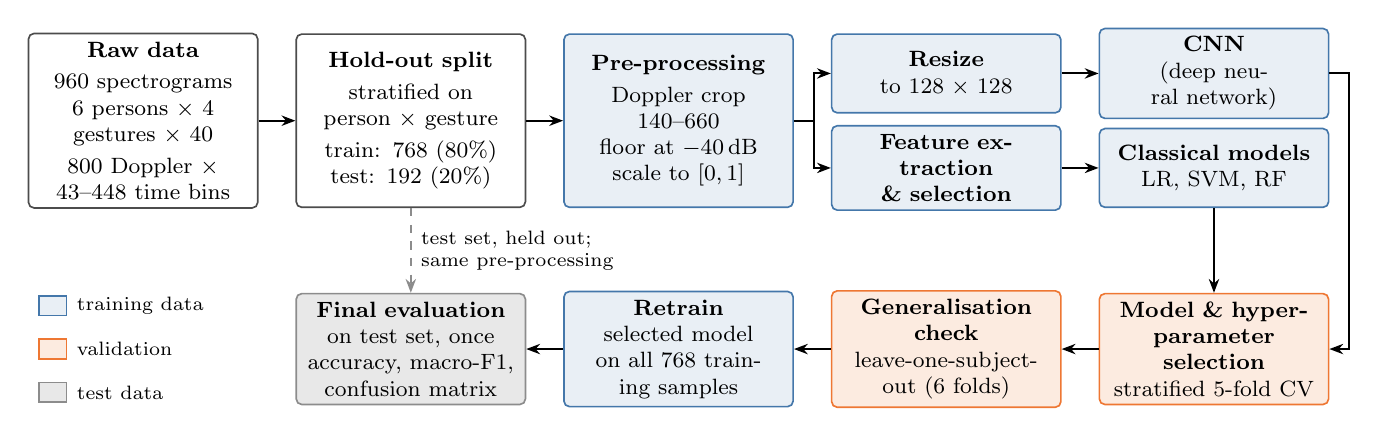
\begin{tikzpicture}[font=\footnotesize,
      box/.style={draw, rounded corners=2pt, align=center, text width=2.7cm,
        inner sep=3pt, line width=0.6pt},
      big/.style={box, minimum height=2.2cm},
      lane/.style={box, minimum height=1.0cm},
      low/.style={box, minimum height=1.4cm},
      data/.style={draw=black!70, fill=white},
      train/.style={draw=trainc, fill=trainc!12},
      val/.style={draw=valc, fill=valc!15},
      test/.style={draw=testc, fill=testc!20},
      arr/.style={-{Stealth[length=5pt]}, line width=0.7pt},
      sw/.style={draw, line width=0.6pt, minimum width=0.35cm, minimum height=0.25cm}]

    % ---- row 1: data -> split -> pre-processing -> two model branches ----
    \node[big, data]  (raw)   at (1.45, 0) {\textbf{Raw data}\\[2pt]
      960 spectrograms\\ 6 persons $\times$ 4 gestures $\times$ 40\\[2pt]
      800 Doppler $\times$ 43--448 time bins};
    \node[big, data]  (split) at (4.85, 0) {\textbf{Hold-out split}\\[2pt]
      stratified on\\ person $\times$ gesture\\[2pt]
      train: 768 (80\%)\\ test: 192 (20\%)};
    \node[big, train] (prep)  at (8.25, 0) {\textbf{Pre-processing}\\[2pt]
      Doppler crop 140--660\\ floor at $-40$\,dB\\ scale to $[0,1]$};
    \node[lane, train] (resize) at (11.65,  0.6) {\textbf{Resize}\\ to $128 \times 128$};
    \node[lane, train] (feat)   at (11.65, -0.6) {\textbf{Feature extraction\\ \& selection}};
    \node[lane, train] (cnn)    at (15.05,  0.6) {\textbf{CNN}\\ (deep neural network)};
    \node[lane, train] (clf)    at (15.05, -0.6) {\textbf{Classical models}\\ LR, SVM, RF};

    % ---- row 2 (right to left): selection -> LOSO -> retrain -> test ----
    \node[low, val]   (cv)      at (15.05, -2.9) {\textbf{Model \& hyper-\\parameter selection}\\
      stratified 5-fold CV};
    \node[low, val]   (loso)    at (11.65, -2.9) {\textbf{Generalisation check}\\
      leave-one-subject-out (6 folds)};
    \node[low, train] (retrain) at (8.25, -2.9) {\textbf{Retrain}\\
      selected model on all 768 training samples};
    \node[low, test]  (eval)    at (4.85, -2.9) {\textbf{Final evaluation}\\
      on test set, once\\ accuracy, macro-F1, confusion matrix};

    % ---- arrows ----
    \draw[arr] (raw) -- (split);
    \draw[arr] (split) -- (prep);
    \draw[arr] (prep.east) -- ++(0.25, 0) |- (resize.west);
    \draw[arr] (prep.east) -- ++(0.25, 0) |- (feat.west);
    \draw[arr] (resize) -- (cnn);
    \draw[arr] (feat) -- (clf);
    \draw[arr] (cnn.east) -- ++(0.25, 0) |- (cv.east);
    \draw[arr] (clf) -- (cv);
    \draw[arr] (cv) -- (loso);
    \draw[arr] (loso) -- (retrain);
    \draw[arr] (retrain) -- (eval);
    % test set bypasses all training and tuning
    \draw[arr, testc, dashed] (split) -- (eval)
      node[midway, right, align=left, font=\scriptsize, text=black]
      {test set, held out;\\ same pre-processing};

    % ---- legend ----
    \node[sw, train] (l1) at (0.3, -2.35) {};
    \node[anchor=west, font=\scriptsize] at (l1.east) {training data};
    \node[sw, val]   (l2) at (0.3, -2.9) {};
    \node[anchor=west, font=\scriptsize] at (l2.east) {validation};
    \node[sw, test]  (l3) at (0.3, -3.45) {};
    \node[anchor=west, font=\scriptsize] at (l3.east) {test data};
  \end{tikzpicture}
  \caption{Overview of the machine learning pipeline. The test set is
    separated before any analysis and is used only once, for the final
    evaluation. All pre-processing constants are chosen from the training
    samples only and applied to each sample separately. The CNN uses the
    resized spectrograms; the classical models use features computed on the
    spectrograms at their original length.}
  \label{fig:pipeline}
\end{figure}

% ---------- Data split: stratified hold-out test set ----------
\begin{figure}[H]
  \centering
  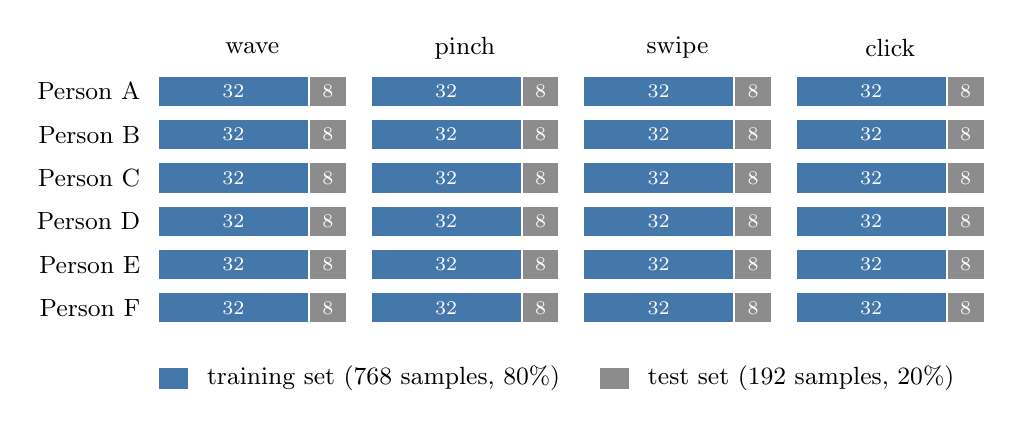
\begin{tikzpicture}[font=\small,
      seg/.style={draw=white, line width=0.8pt},
      lab/.style={font=\scriptsize, text=white}]
    % gesture column headers
    \foreach \g [count=\j from 0] in {wave, pinch, swipe, click}
      \node at ({\j*2.7+1.2}, 0.35) {\g};
    % one bar per person x gesture: 32 training (80%) + 8 test (20%)
    \foreach \p [count=\i from 0] in {A, B, C, D, E, F} {
      \node[anchor=east] at (-0.1, {-\i*0.55-0.2}) {Person \p};
      \foreach \j in {0,...,3} {
        \filldraw[seg, fill=trainc] ({\j*2.7}, {-\i*0.55}) rectangle ++(1.92, -0.4);
        \node[lab] at ({\j*2.7+0.96}, {-\i*0.55-0.2}) {32};
        \filldraw[seg, fill=testc] ({\j*2.7+1.92}, {-\i*0.55}) rectangle ++(0.48, -0.4);
        \node[lab] at ({\j*2.7+2.16}, {-\i*0.55-0.2}) {8};
      }
    }
    % legend
    \filldraw[seg, fill=trainc] (0, -3.7) rectangle ++(0.4, -0.3);
    \node[anchor=west] at (0.5, -3.85) {training set (768 samples, 80\%)};
    \filldraw[seg, fill=testc] (5.6, -3.7) rectangle ++(0.4, -0.3);
    \node[anchor=west] at (6.1, -3.85) {test set (192 samples, 20\%)};
  \end{tikzpicture}
  \caption{Stratified hold-out test set. Each of the 24 person--gesture
    combinations has 40 samples, of which 8 are assigned to the test set, so
    the test set has the same class and person balance as the full dataset.
    The test set is separated before any pre-processing and used only once,
    for the final evaluation.}
  \label{fig:split-stratified}
\end{figure}

% ---------- Data split: cross-validation folds ----------
\begin{figure}[H]
  \centering
  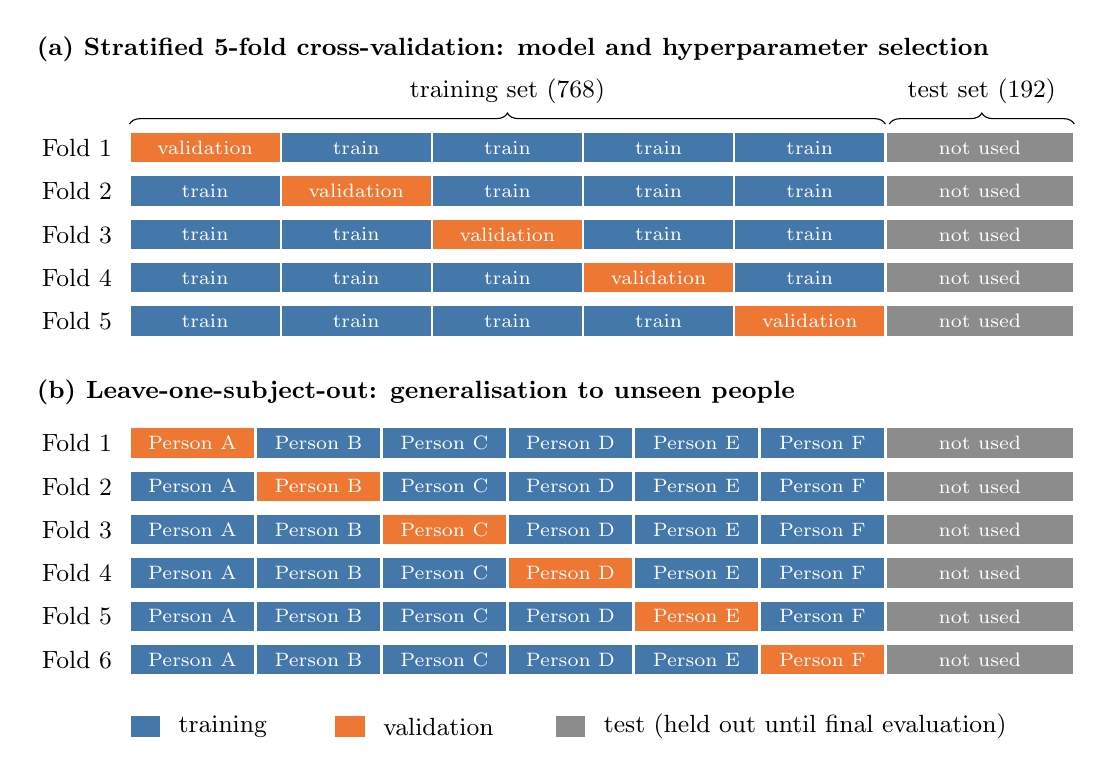
\begin{tikzpicture}[font=\small,
      seg/.style={draw=white, line width=0.8pt},
      lab/.style={font=\scriptsize, text=white}]
    % ---- (a) stratified 5-fold ----
    \node[anchor=west, font=\small\bfseries] at (-1.3, 1.05)
      {(a) Stratified 5-fold cross-validation: model and hyperparameter selection};
    \draw[decorate, decoration={brace, amplitude=4pt}] (0, 0.1) -- (9.6, 0.1)
      node[midway, above=4pt] {training set (768)};
    \draw[decorate, decoration={brace, amplitude=4pt}] (9.65, 0.1) -- (12, 0.1)
      node[midway, above=4pt] {test set (192)};
    \foreach \k in {1,...,5} {
      \pgfmathsetmacro{\y}{-(\k-1)*0.55}
      \node[anchor=east] at (-0.1, \y-0.2) {Fold \k};
      \foreach \s in {1,...,5} {
        \ifnum\s=\k \def\segcol{valc}\def\seglab{validation}%
        \else \def\segcol{trainc}\def\seglab{train}\fi
        \filldraw[seg, fill=\segcol] ({(\s-1)*1.92}, \y) rectangle ++(1.92, -0.4);
        \node[lab] at ({(\s-1)*1.92+0.96}, \y-0.2) {\seglab};
      }
      \filldraw[seg, fill=testc] (9.6, \y) rectangle ++(2.4, -0.4);
      \node[lab] at (10.8, \y-0.2) {not used};
    }
    % ---- (b) leave-one-subject-out ----
    \node[anchor=west, font=\small\bfseries] at (-1.3, -3.3)
      {(b) Leave-one-subject-out: generalisation to unseen people};
    \foreach \p [count=\k] in {A, B, C, D, E, F} {
      \pgfmathsetmacro{\y}{-3.75-(\k-1)*0.55}
      \node[anchor=east] at (-0.1, \y-0.2) {Fold \k};
      \foreach \q [count=\s] in {A, B, C, D, E, F} {
        \ifnum\s=\k \def\segcol{valc}\else \def\segcol{trainc}\fi
        \filldraw[seg, fill=\segcol] ({(\s-1)*1.6}, \y) rectangle ++(1.6, -0.4);
        \node[lab] at ({(\s-1)*1.6+0.8}, \y-0.2) {Person \q};
      }
      \filldraw[seg, fill=testc] (9.6, \y) rectangle ++(2.4, -0.4);
      \node[lab] at (10.8, \y-0.2) {not used};
    }
    % legend
    \filldraw[seg, fill=trainc] (0, -7.4) rectangle ++(0.4, -0.3);
    \node[anchor=west] at (0.5, -7.55) {training};
    \filldraw[seg, fill=valc] (2.6, -7.4) rectangle ++(0.4, -0.3);
    \node[anchor=west] at (3.1, -7.55) {validation};
    \filldraw[seg, fill=testc] (5.4, -7.4) rectangle ++(0.4, -0.3);
    \node[anchor=west] at (5.9, -7.55) {test (held out until final evaluation)};
  \end{tikzpicture}
  \caption{Validation folds on the training set (768 samples). (a)~Stratified
    5-fold cross-validation: every training sample is used for validation
    exactly once, and each fold keeps the class balance; the model and
    hyperparameters with the best mean validation score are selected.
    (b)~Leave-one-subject-out: the chosen model is trained on five people and
    validated on the sixth, which measures generalisation to people not seen
    during training. In both schemes the test set is never used.}
  \label{fig:split-folds}
\end{figure}

\newpage
% =====================================================================
\section{Task 1: Data Pre-processing and Feature Extraction}
\label{sec:task1}
% =====================================================================
% \placeholder{%
% \textbf{Required content:} selected options for pre-processing and possible
% feature extraction, \emph{argumentation for the selection}, and
% \emph{results}. \textbf{Rubric: Data analysis \& pre-processing (10\%) +
% Feature selection (15\%).} Explain the implementation without showing complete
% code; short key code steps are acceptable.}

\subsection{Exploratory Data Analysis}
The exploratory data analysis has been conducted using only samples from the training set. This prevents leakage from the test set into the processing choices.
% \placeholder{%
% \begin{itemize}
%   \item Example spectrogram per class (magnitude in dB) -- one figure with 4
%         subplots, labelled axes (Doppler/velocity bin, time), colourbar.
%   \item Statistics: number of samples per class and per person, distribution
%         of spectrogram lengths, dynamic range of dB values, outliers / corrupt
%         or empty samples (NaN, inf, all-zero), inter-subject variability.
%   \item Observations that motivate the pre-processing choices below.
% \end{itemize}}
\begin{figure}[H]
  \centering
  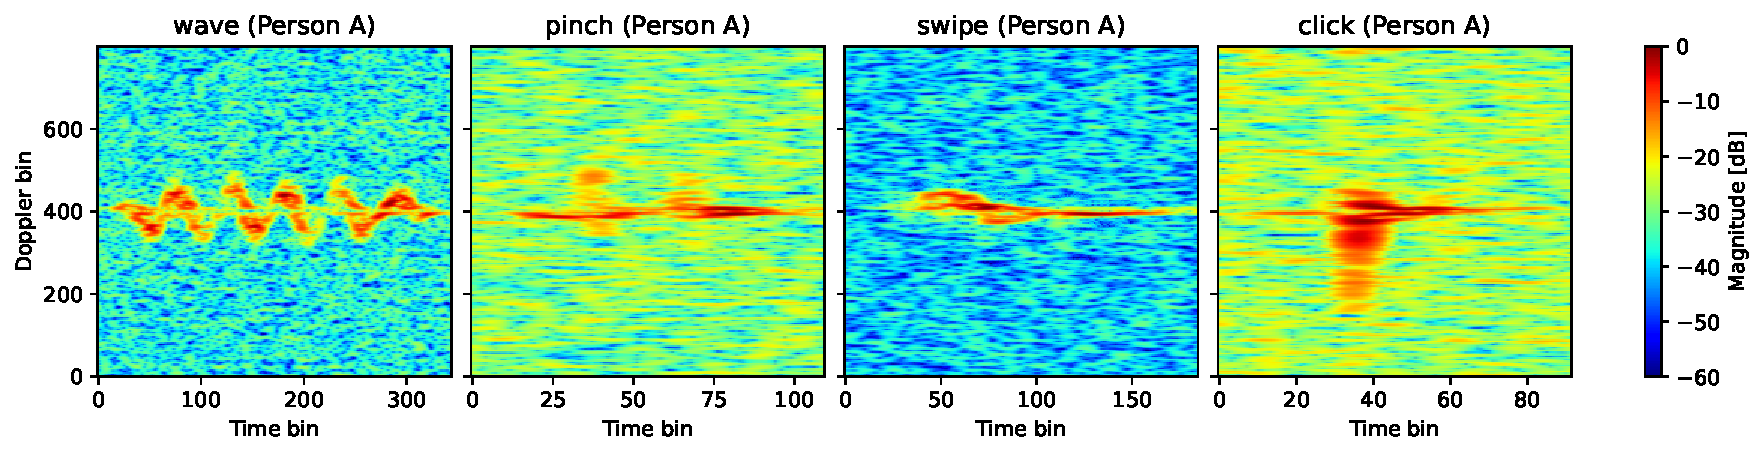
\includegraphics[width=\linewidth]{figures/spectrograms.pdf}
  \caption{Example micro-Doppler spectrogram for each gesture (magnitude in dB).}
  \label{fig:spectrograms}
\end{figure}
\begin{wrapfigure}{r}{0.35\linewidth}  % [11] = number of narrowed lines; tweak 9–13
  \centering
  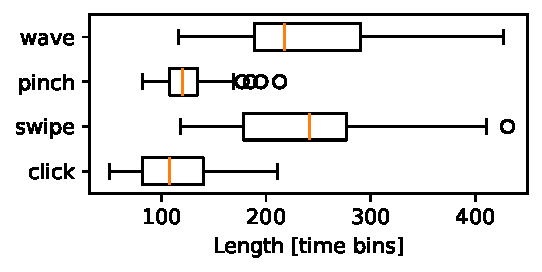
\includegraphics[width=\linewidth]{figures/length_boxplot.pdf}
  \caption{Sample length per gesture.}
  \label{fig:length_boxplot}
\end{wrapfigure}
\noindent
The spectrograms all share a similar structure with 800 doppler bins and a varying number of time bins. An example spectogram of each of the 4 gestures is presented in \autoref{fig:spectrograms}. Zero motion is placed in the centre at doppler bin 400. The spectograms have already been cropped to the gesture duration, which causes the varying number of time bins between samples. Wave and swipe gestures tend to take longer than click and pinch gestures, as shown in \autoref{fig:length_boxplot}. The sample duration therefore holds relevant information that would be removed by resizing all spectrograms to equal length.
\\\\
 Yet, the spectrograms have varying magnitude ranges depending on both the gesture and the person. Most of the values however contain background noise instead of gesture energy. The background noise level differs per sample, as seen in \autoref{fig:doppler_profile_persons}, making a fixed noise floor for all samples unsuitable. 
\begin{figure}[H]
    \centering
    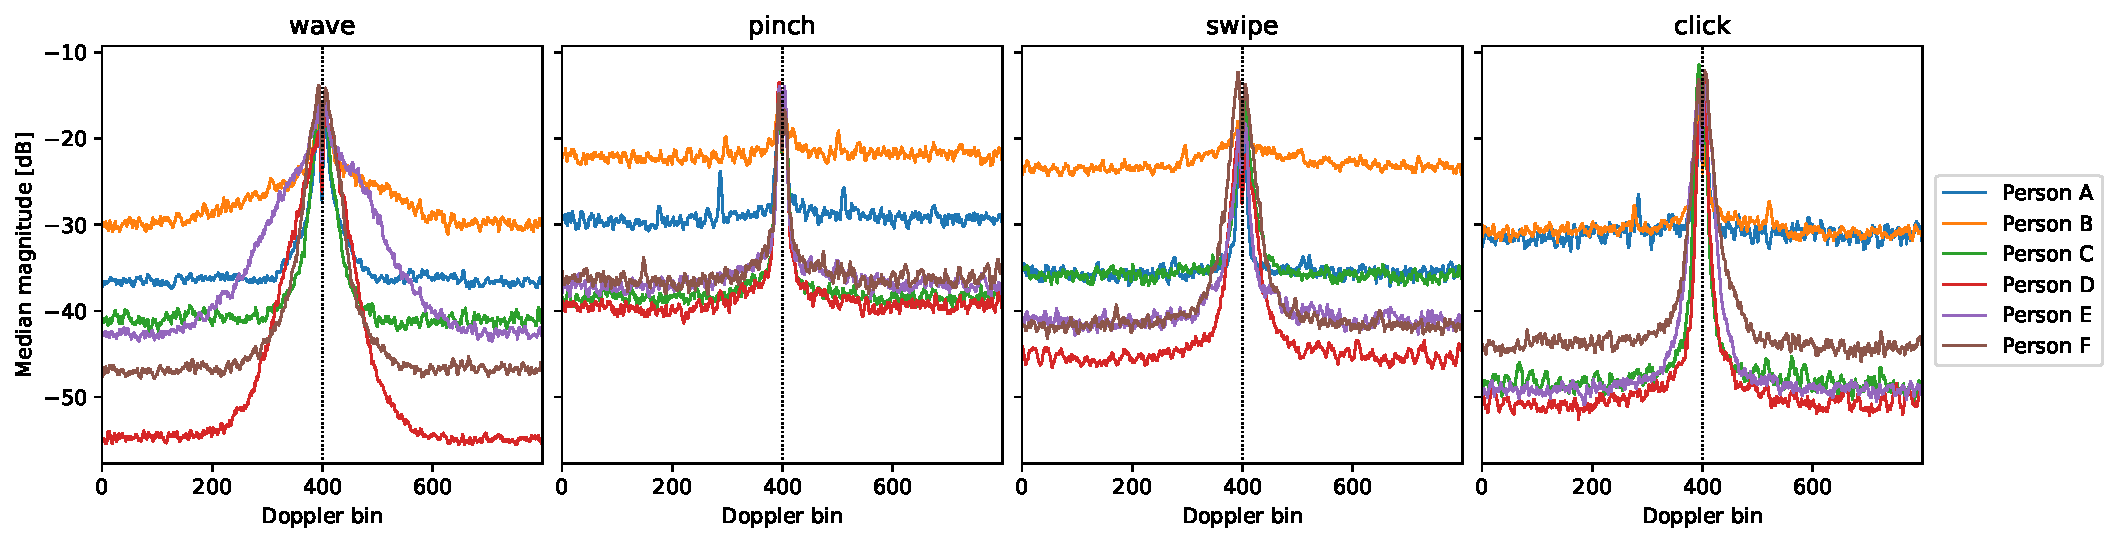
\includegraphics[width=\linewidth]{figures/doppler_profile_persons.pdf}
    \caption{Median magnitude per Doppler bin per gesture and person.}
    \label{fig:doppler_profile_persons}
\end{figure}
\noindent
The data needs to be made more uniform by removing noise and rescaling such that the model is prevented from learning a gesture mainly based on the background noise level. This also poses a challenge generalizing the model to more people since the model will learn person specific features with just 6 people in the training data. The gestures should be distinguished on the distribution of gesture energy over time and doppler bins.

\subsection{Pre-processing}
Since there are no invalid values in the provided dataset, no samples have to be removed. All samples will be processed in four steps: noise removal, cropping, scaling and resizing. The goal of the pre-processing is to make turn the raw data into clean spectograms of uniform dimensions, that can be used for feature extraction and model training.

\begin{figure}[H]
  \centering
  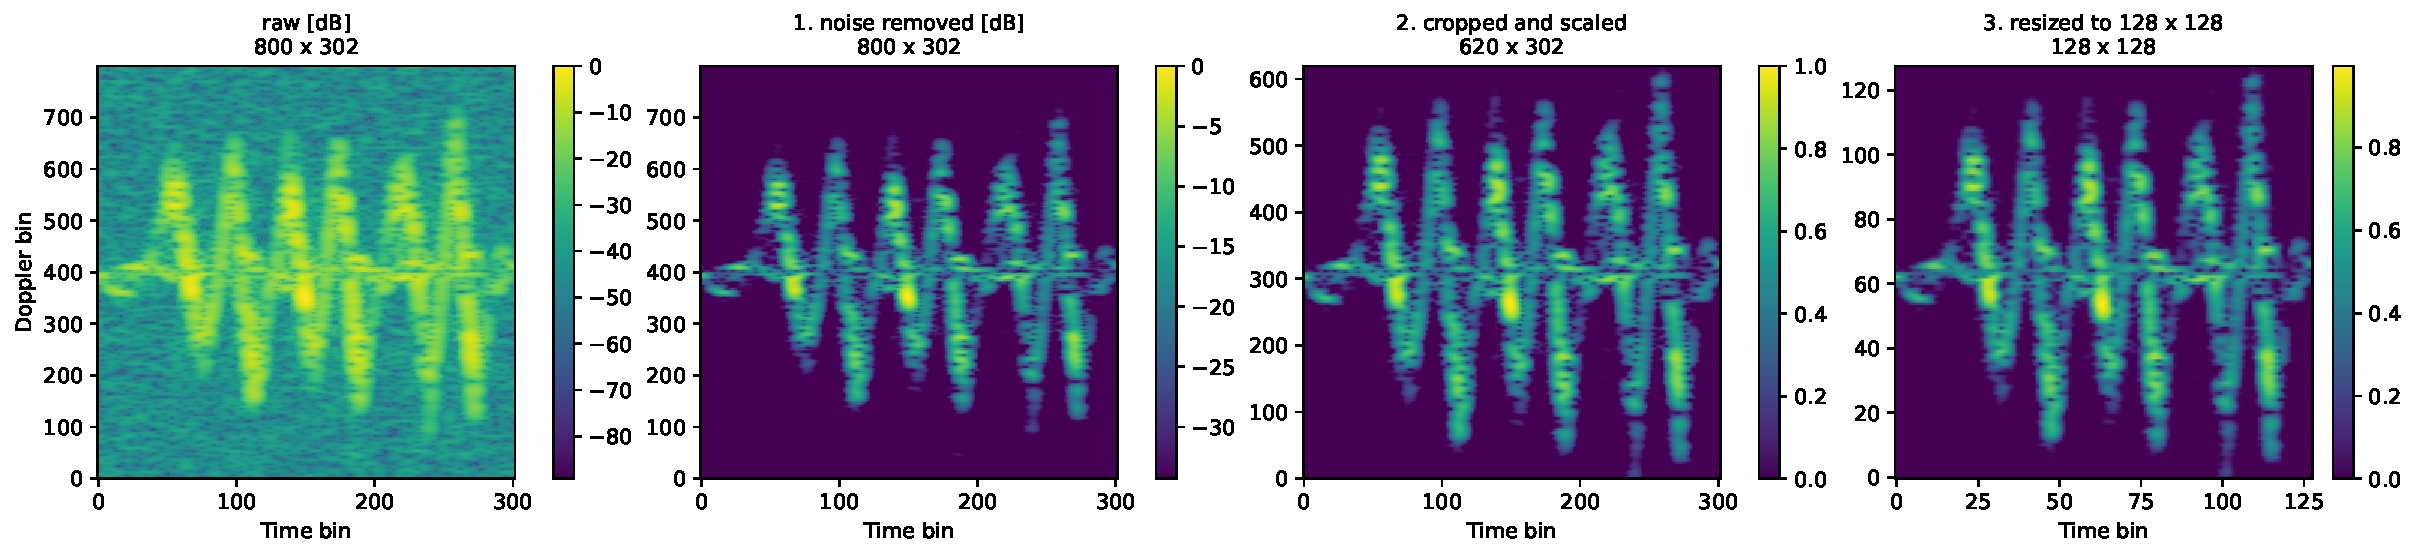
\includegraphics[width=\linewidth]{figures/prepro_all_steps.pdf}
  \caption{The four pre-processing steps applied to one wave sample from the training set. The size of the image (Doppler $\times$ time bins) is given above each panel.}
  \label{fig:prepro_steps}
\end{figure}

\paragraph{Noise removal} As shown before in \autoref{fig:doppler_profile_persons}, the samples all have their own noise floor level. This background noise can be removed since it contains no useful information about the gesture. Because of the sample specific noise floor, the noise removal process also has to be sample specific. A fixed clip for example would leave cut into the gesture of some samples, while leaving noise in others. Since the gesture mainly takes places in the bins close to zero Doppler, the bins far away from the centre mainly consist of noise. Therefore, the sample noise floor level is determined using the median value of the far bins. The median is well suited for this, rather than the mean, since it is less sensitive to a few bins that contain the gesture. As long as more than half of the time bins contain noise, the median gives a good estimate of the noise level. The far bins range is chosen to be Doppler bins 0-50 and 750-800 based on TODO why these bins? Since the far bins contain mostly noise, using the median as noise floor would only remove half of the noise. Therefore, a margin is added on top of the noise floor such that 99\% of the noise is removed. This margin is a trade-off between removing more noise and preserving gesture information. For each sample, all values are clipped at the sample specific noise floor plus that fixed margin.

\paragraph{Cropping}
Since the far bins contain mainly noise and hold little gesture information, they might as well be removed to improve the Doppler resolution when resizing the spectrogram later on. However, only bins that do not contain gesture information should be removed. For 99\% of the samples, the gesture energy lies within the bins 100-800. A narrower crop would give a higher resolution after resizing, at the cost of removing the tails of gestures that do reach into the far bins.

\paragraph{Scaling}
After the noise removal, each sample still has a different noise floor. The model should not learn the gestures based on this noise floor. The sample dependent noise floor should therefore be converted to a uniform noise floor. This is done using per sample scaling. The noise floor becomes zero, since it has no information and the maximum (0 dB) becomes 1.

\paragraph{Resizing}
Finally, the spectrograms have to made uniform in their dimensions so that they can be used as input for a CNN. A resolution of 128 x 128 is chosen as the output size. The spectrograms are all resized using linear interpolation. This does remove gesture duration, which did hold relevant information so that will be added as a separate feature later on.


% \placeholder{%
% Describe and \emph{justify} each step chosen (the assignment lists data
% cleaning, normalisation, standardisation of spectrograms treated as images).
% Examples to consider:
% \begin{itemize}
%   \item Data cleaning: handling NaN/inf, removing corrupted samples.
%   \item Handling variable time length: cropping, zero/min-padding, resizing /
%         interpolation to a fixed size.
%   \item Dynamic-range clipping (e.g.\ floor at max$-X$\,dB) to suppress noise.
%   \item Normalisation / standardisation (per-sample min--max, global z-score
%         fitted on training data only -- avoid leakage).
%   \item Optional: Doppler cropping around zero velocity, denoising, data
%         augmentation for the DNN (time shift, noise) -- training set only.
% \end{itemize}
% Report the effect of each choice (figure before/after, and/or ablation
% showing impact on validation accuracy).}
% TODO why we picked zoom and not zero padding or interpolation




\begin{figure}[H]
  \centering
  \begin{subfigure}{\linewidth}
    \centering
    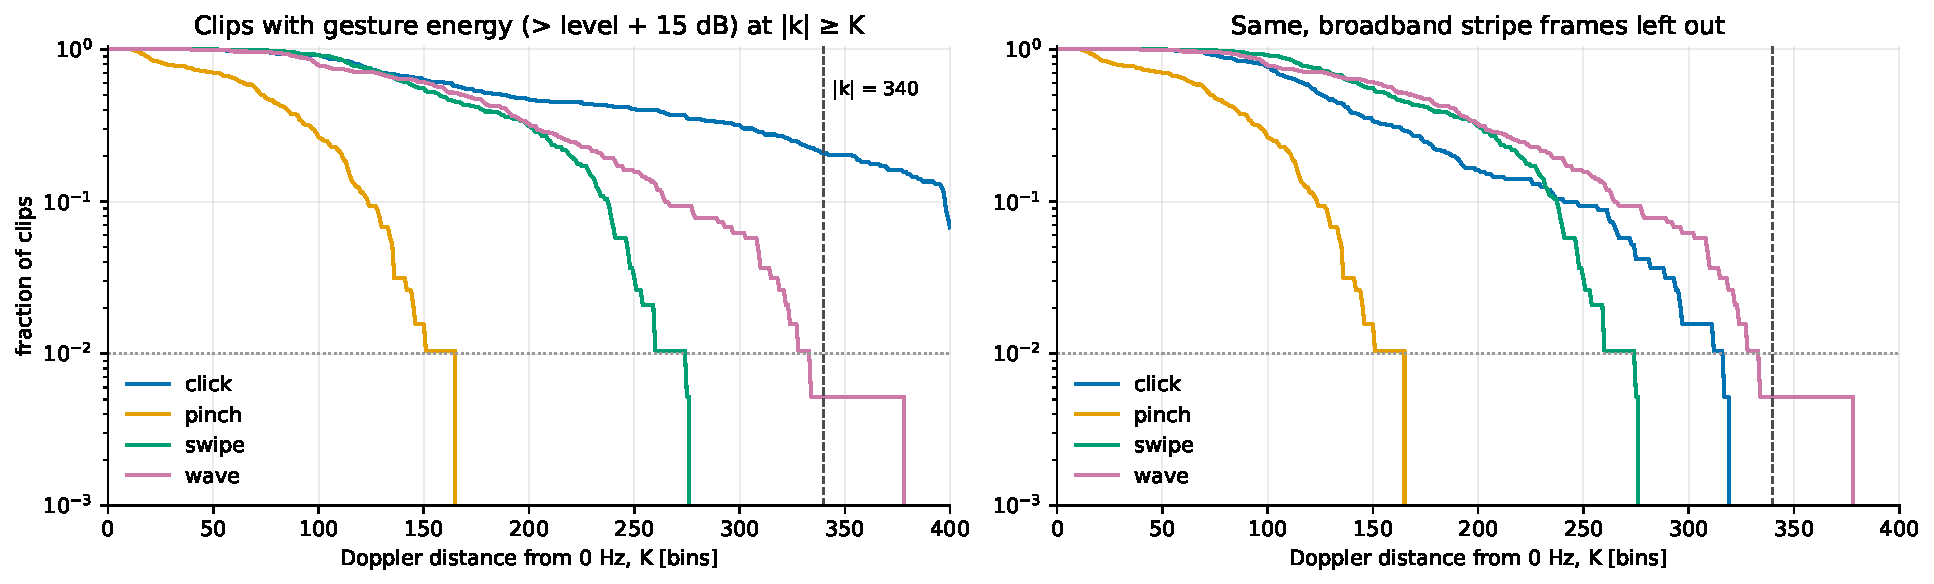
\includegraphics[width=\linewidth]{figures/noise_far_bins.pdf}
    \caption{Fraction of training samples with gesture energy at a Doppler distance of at least $K$ bins. Left: all time frames; right: broadband click stripes left out. The dashed line marks the far-bin boundary $|k| = 340$.}
    \label{fig:noise_far_bins}
  \end{subfigure}
  \\[4pt]
  \begin{subfigure}{\linewidth}
    \centering
    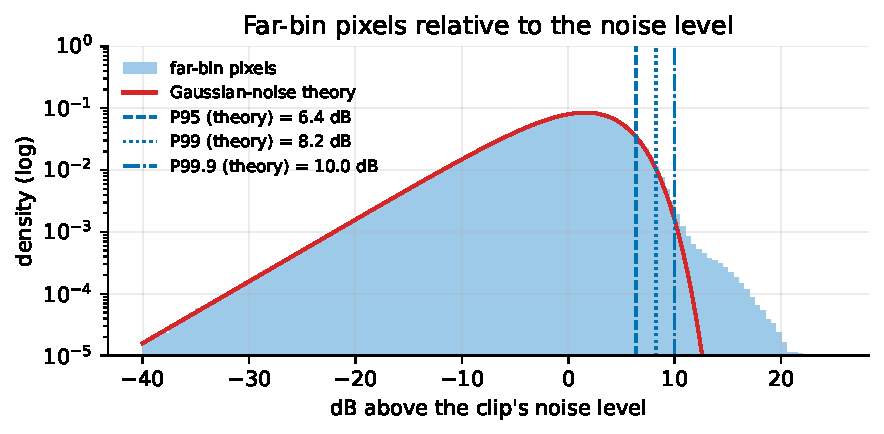
\includegraphics[width=\linewidth]{figures/noise_margin.pdf}
    \caption{Left: distribution of far-bin pixels relative to each sample's noise level, with the Rayleigh-noise theory. Right: share of noise pixels that remain above the threshold as a function of the margin.}
    \label{fig:noise_margin}
  \end{subfigure}
  \caption{Choice of the far bins (a) and the noise margin (b), derived on the training samples.}
  \label{fig:noise_params}
\end{figure}

\subsection{Feature Extraction and Selection}
\placeholder{%
Optional in the assignment but worth \textbf{15\%} of the rubric -- argue why
you do/do not use explicit features (e.g.\ DNN on raw images vs.\ handcrafted
features for classical models). Inspiration suggested by the lecturer:
\begin{enumerate}
  \item \textbf{Envelope features} -- Amin, Zeng \& Shan, \emph{Hand Gesture
        Recognition based on Radar Micro-Doppler Signature Envelopes}, IEEE
        RadarConf 2019 \cite{amin2019}: upper/lower/central envelopes of the
        spectrogram.
  \item \textbf{Centroid and bandwidth} -- Fioranelli, Ritchie \& Griffiths,
        IET RSN 2016 \cite{fioranelli2016}, Sec.~3.2: Doppler centroid and
        bandwidth over time and their statistical moments (note: originally for
        a different task).
  \item \textbf{Chebyshev moments} -- Pallotta et al., IEEE MetroAeroSpace 2021
        \cite{pallotta2021}.
\end{enumerate}
Other options: statistical features (mean, variance, skewness, kurtosis,
energy, entropy), PCA, image-texture features. Explain:
\begin{itemize}
  \item Feature definitions (equations where useful).
  \item Feature selection / dimensionality reduction method (e.g.\ correlation
        analysis, mutual information, recursive feature elimination, PCA
        explained variance) and why.
  \item Results: feature distributions per class, separability plots
        (e.g.\ pair plots, t-SNE/PCA scatter), feature importance ranking.
\end{itemize}}

\begin{table}[H]
  \centering
  \caption{Extracted features (example layout).}
  \label{tab:features}
  \begin{tabular}{@{}llc@{}}
    \toprule
    Feature group & Description & \# features \\
    \midrule
    Envelope        & \ldots & -- \\
    Centroid/bandwidth & \ldots & -- \\
    Chebyshev moments  & \ldots & -- \\
    \bottomrule
  \end{tabular}
\end{table}

\subsection{Task 1 Results}
\placeholder{%
Summarise the outcome of Task~1: final input representation(s) fed to each
model, final feature set and its size, key plots showing class separability,
and a short discussion of what worked and what did not.}

% =====================================================================
\section{Task 2: Model Development, Validation and Comparison}
\label{sec:task2}
% =====================================================================
\subsection{Model Selection and Design}
\label{sec:models}
Five models are tested on the pre-processed data of Task~1: three on the 27
hand-crafted features and two on the $128 \times 128$ spectrogram images.
\begin{itemize}
  \item \textbf{Logistic regression (LR):} multinomial (softmax) model trained
        with the cross-entropy loss and an L2 penalty; the linear,
        interpretable baseline.
  \item \textbf{SVM (features):} soft-margin support vector machine; a linear,
        polynomial or RBF kernel allows a nonlinear decision boundary.
  \item \textbf{Random forest (RF):} decision trees, each trained on a bootstrap
        sample with a random subset of features per split, combined by
        majority vote; needs no scaling and captures feature interactions.
  \item \textbf{SVM + PCA (images):} PCA with whitening reduces the 16\,384
        pixels to at most 100 components, followed by an SVM; tests whether
        raw pixels can replace hand-crafted features.
  \item \textbf{CNN (images):} the required deep network, which learns its own
        features from the images.
\end{itemize}
Scaling and PCA are part of a scikit-learn \texttt{Pipeline}, so they are
fitted on the training folds only.

\subsubsection{CNN layout}
The CNN (\cref{tab:cnn-layout}) consists of convolution
blocks, each a $3 \times 3$ convolution with ReLU activation followed by
$2 \times 2$ max pooling, then dropout (0.5) and a softmax layer with one output
per gesture. The convolutions use zero padding: a convolution
keeps the size of its input and only the pooling halves it, so after five blocks
the image is exactly $4 \times 4$. Without padding every convolution would also
remove the outer pixels, which hold the start and end of a gesture and the
highest Doppler velocities. ReLU, $\max(0, x)$, does not saturate for positive
inputs, so the gradient does not vanish through the five layers, and it is cheap
to compute; its sparse output also suits the spectrograms, in which most pixels
are zero after noise removal. With 26\,436 parameters the network is small
enough for 960 samples. It is trained with the cross-entropy loss and mini-batch
SGD (batch size 32); training stops when the loss on 10\% of the training data
has not decreased for 10 epochs.

\begin{table}[!htbp]
  \centering
  \caption{Selected CNN layout ($3 \times 3$ convolutions, zero padding, ReLU).}
  \label{tab:cnn-layout}
  \small
  \begin{tabular}{@{}llr@{}}
    \toprule
    Layer & Output shape & Parameters \\
    \midrule
    Input (spectrogram)            & $128 \times 128 \times 1$ & 0 \\
    Block 1: conv (8) + max pool   & $64 \times 64 \times 8$   & 80 \\
    Block 2: conv (16) + max pool  & $32 \times 32 \times 16$  & 1\,168 \\
    Block 3: conv (32) + max pool  & $16 \times 16 \times 32$  & 4\,640 \\
    Block 4: conv (32) + max pool  & $8 \times 8 \times 32$    & 9\,248 \\
    Block 5: conv (32) + max pool  & $4 \times 4 \times 32$    & 9\,248 \\
    Flatten + dropout (0.5)        & 512                       & 0 \\
    Dense + softmax                & 4                         & 2\,052 \\
    \midrule
    Total                          &                           & 26\,436 \\
    \bottomrule
  \end{tabular}
\end{table}

\subsection{Validation Procedure and Performance Indicators}
\label{sec:validation}
Every model is validated in two ways:
\begin{itemize}
  \item \textbf{Leave-one-subject-out (LOSO):} six folds, each trained on five
        persons and validated on the sixth. This measures recognition of a
        person not seen during training, the aim of the project. The LOSO
        accuracy is the mean over the six persons of the best hyperparameter
        setting; because the same folds choose and score the setting, it is
        slightly optimistic.
  \item \textbf{Random split:} the 80/20 split of
        \cref{fig:pipeline}. The hyperparameters are chosen with 5-fold
        cross-validation on the 768 training samples (validation accuracy); the
        best settings are saved and tested once on the 192
        test samples.
\end{itemize}
The 40 repetitions per person and gesture come from one recording, so in a
random split the same person appears in training and validation. The classes
are balanced, so accuracy is the main metric, together with macro-averaged
precision, recall and F1 and by confusion matrices.

\subsection{Hyperparameter Tuning}
\label{sec:tuning}
All models are tuned with a grid search: every setting is trained on the
training folds and the one with the highest mean validation accuracy is
selected, separately for LOSO and for the random split (\cref{tab:hyper}).
\Cref{fig:tuning} shows the training and validation accuracy along the most
important hyperparameter of the classical models.

\begin{table}[!htbp]
  \centering
  \caption{Hyperparameter search space and selected values.}
  \label{tab:hyper}
  \small
  \begin{tabular}{@{}llll@{}}
    \toprule
    Model & Search space & LOSO & Random split \\
    \midrule
    LR             & $C$: $10^{-3}, 10^{-2}, \dots, 10^{3}$ & $C = 10$ & $C = 1$ \\
    SVM (features) & kernel: linear/poly/RBF; $C$: 0.1, 1, 10, 100 & linear, $C = 1$ & RBF, $C = 10$ \\
    SVM + PCA      & components: 20/50/100; kernel; $C$ & 20, RBF, $C = 1$ & 20, RBF, $C = 10$ \\
    RF             & trees: 50/100/300; depth: 3/5/10/$\infty$ & 300, depth 10 & 100, depth $\infty$ \\
    CNN            & blocks: 4, 5, 6, \dots\ (until LOSO drops) & 5 blocks & 5 blocks \\
    \bottomrule
  \end{tabular}
\end{table}

\begin{figure}[H]
  \centering
  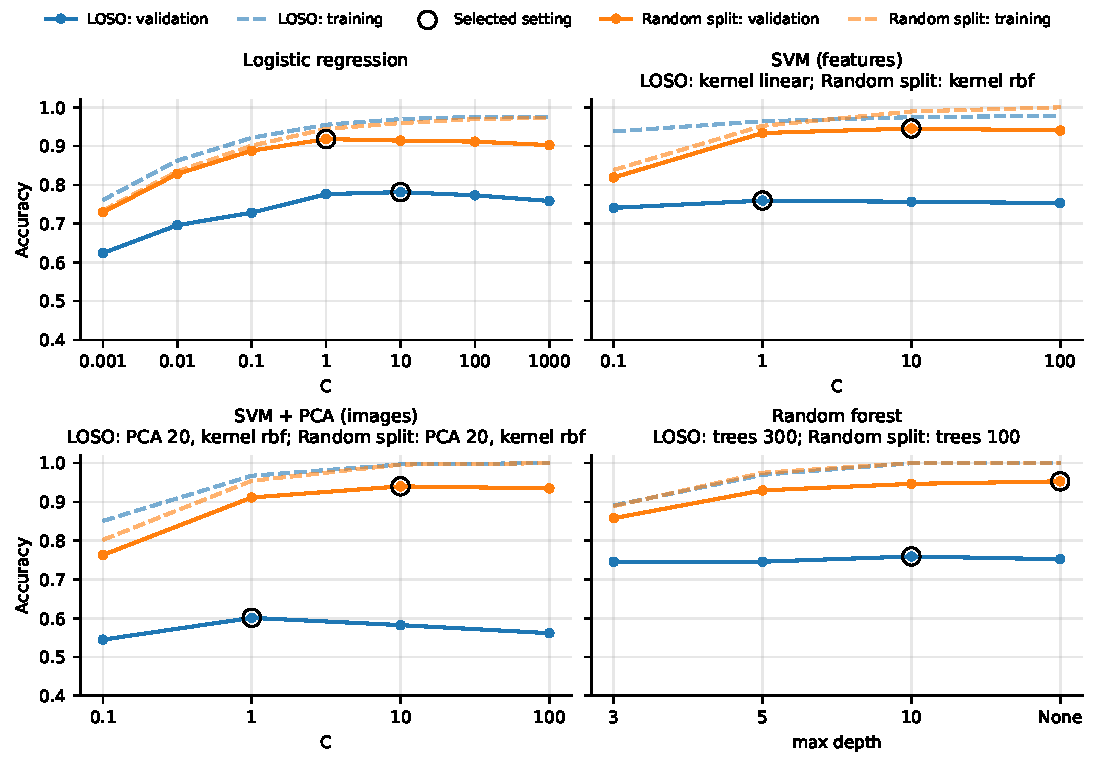
\includegraphics[width=0.85\linewidth]{figures/report_tuning.pdf}
  \caption{Training (dashed) and validation (solid) accuracy per hyperparameter; circles: selected setting.}
  \label{fig:tuning}
\end{figure}

\subsubsection{Classical models}
Three observations follow from \cref{fig:tuning}.
First, under LOSO the validation accuracy stays 0.14--0.42 below the training
accuracy for every setting: the limit is the generalisation to a new person, not
the fit. Second, the random split selects more flexible settings than LOSO
(\cref{tab:hyper}): an RBF kernel with $C = 10$ instead of a linear kernel for
the SVM, and fully grown trees for the RF. A random split rewards memorising
person-specific details, because the same person is in the training and
validation folds. Third, LR improves up to $C = 10$ (0.78) and drops slightly
with weaker regularisation (0.76 at $C = 1000$), and SVM + PCA does not exceed
0.60 under LOSO, against 0.94 for the random split.

\subsubsection{CNN layout search}
For the CNN the number of convolution blocks is the
most important hyperparameter. Starting at four blocks, one block of 32 filters
is added at a time until the LOSO validation accuracy goes down
(\cref{fig:cnn-depth}). The learning rate and dropout are fixed at 0.03 and 0.5,
the values chosen in an earlier nested search on the previous pre-processing
(dropout 0.5 in five of six folds, learning rates 0.01--0.1). Four blocks reach
0.67, five 0.73 and six 0.69, so five blocks are selected. The training accuracy
is 0.98--0.99 for every depth, so the depth changes the generalisation, not the
fit. Each block halves the feature map and enlarges the receptive field: with
four blocks a unit sees 46 of the 128 pixels, with five blocks 94, which covers
most of a gesture. A sixth block adds parameters (34\,148 versus 26\,436)
without new context. The random split cannot separate five and six blocks (0.96
for both).

\begin{figure}[H]
  \centering
  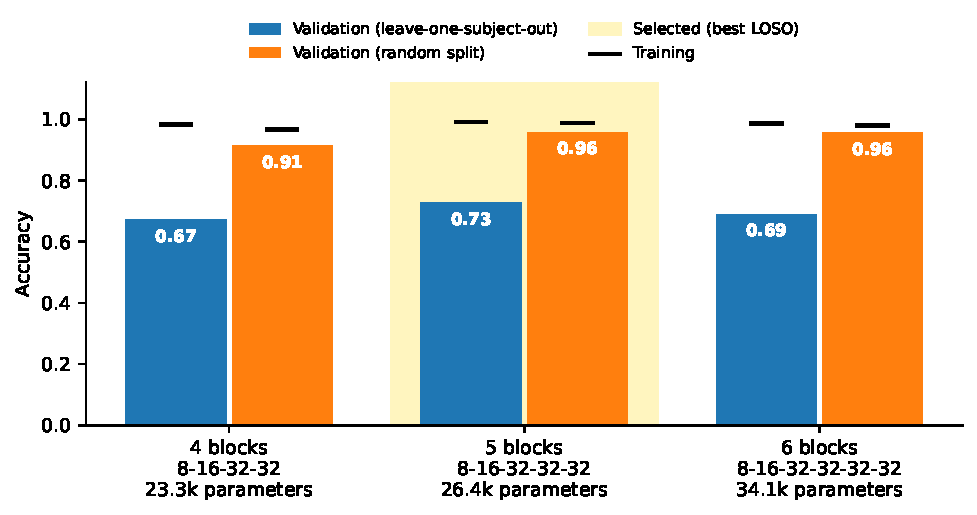
\includegraphics[width=0.7\linewidth]{figures/cnn_depth_search.pdf}
  \caption{CNN depth search: validation (bars) and training (black lines) accuracy.}
  \label{fig:cnn-depth}
\end{figure}

\subsection{Results and Comparison}
\label{sec:results}
\begin{table}[!htbp]
  \centering
  \caption{Accuracy and macro-F1 of the selected settings (LOSO: mean $\pm$ std over six persons; --: not evaluated).}
  \label{tab:results}
  \small
  \begin{tabular}{@{}lccccc@{}}
    \toprule
    & \multicolumn{2}{c}{LOSO} & \multicolumn{3}{c}{Random split} \\
    \cmidrule(lr){2-3} \cmidrule(l){4-6}
    Model & Accuracy & Macro-F1 & Validation & Test & Test macro-F1 \\
    \midrule
    LR                 & $\mathbf{0.781 \pm 0.131}$ & \textbf{0.779} & 0.918 & 0.948 & 0.948 \\
    SVM (features)     & $0.759 \pm 0.139$ & 0.755 & 0.945 & \textbf{0.974} & \textbf{0.974} \\
    RF                 & $0.759 \pm 0.204$ & 0.757 & 0.953 & 0.948 & 0.948 \\
    SVM + PCA (images) & $0.601 \pm 0.135$ & 0.591 & 0.940 & 0.938 & 0.938 \\
    CNN (images)       & $0.727$           & --    & \textbf{0.958} & -- & -- \\
    \bottomrule
  \end{tabular}
\end{table}

\begin{figure}[H]
  \centering
  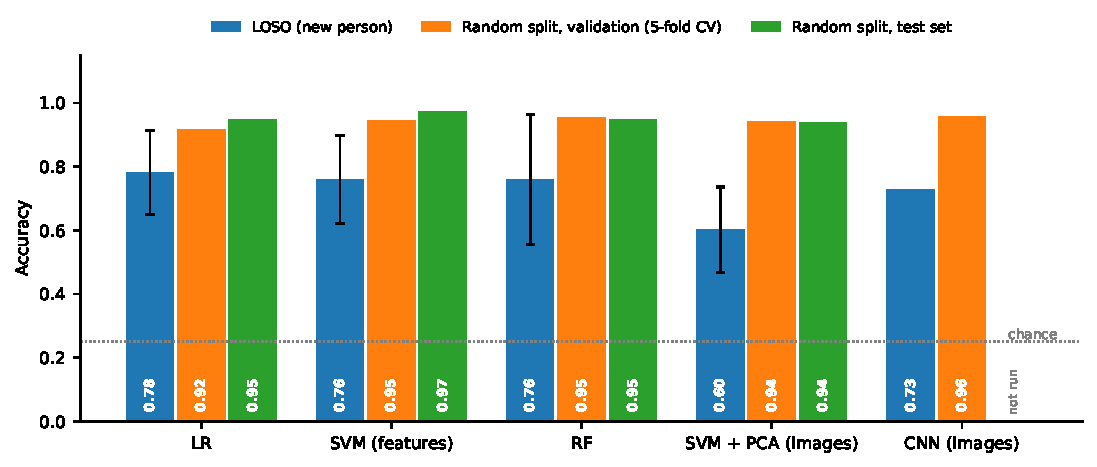
\includegraphics[width=0.78\linewidth]{figures/report_comparison.pdf}
  \caption{Accuracy per model: LOSO (error bars: std over persons), random-split validation and test.}
  \label{fig:comparison}
\end{figure}

\subsubsection{LOSO versus random split}
\Cref{fig:comparison} shows the
results: on the random split all models reach 0.92--0.97, but for a new person
the accuracy drops to 0.60--0.78. The random split overestimates the accuracy by
0.17 (LR) to 0.34 (SVM + PCA) and ranks the models differently: LR is the weakest
on the random-split validation (0.92) but the best under LOSO. The random-split
validation and test accuracies agree within 0.03, so the optimism comes from the
shared persons, not from the size of the test set.

\subsubsection{Comparison of the models}
Under LOSO the three feature models are the
best (LR 0.78, SVM 0.76, RF 0.76), followed by the CNN (0.73) and SVM + PCA
(0.60). The differences between the feature models (at most 0.02) are much
smaller than the spread between persons (std 0.13--0.20), so they are not
significant. Hand-crafted features such as the Doppler centroid, the envelopes
and the duration describe the motion itself and transfer to a new person. On the
same images the CNN is 0.13 better than SVM + PCA: convolution and pooling detect
local patterns at any position, whereas PCA components depend on where a pattern
lies in the image. Macro-F1 is within 0.01 of the accuracy for every model, as
expected for balanced classes.

\begin{figure}[!htbp]
  \centering
  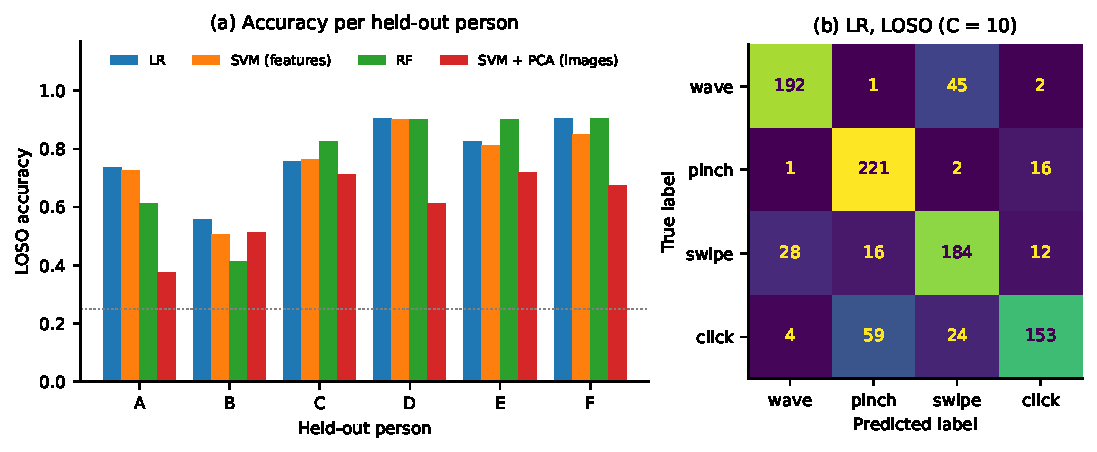
\includegraphics[width=0.8\linewidth]{figures/report_persons.pdf}
  \caption{(a) LOSO accuracy per held-out person. (b) Confusion matrix of LR under LOSO.}
  \label{fig:persons}
\end{figure}

\subsubsection{Errors}
Person B is the hardest for all models (0.41--0.56), while
persons D and F reach 0.85--0.91 with the feature models (\cref{fig:persons}a);
the RF varies most between persons (0.41--0.91). The confusion matrix of LR
(\cref{fig:persons}b) shows the physically similar pairs: 59 of the 240 clicks
are predicted as pinch (click recall 0.64), both short finger movements, and 45
waves as swipe, both long hand movements; pinch is recognised best (0.92).

\subsubsection{Summary}
The random split overestimates the accuracy for a new person
by 0.17--0.34 and cannot separate the models, so the models are compared on
LOSO. LR on the hand-crafted features is the final model: it has the best LOSO
accuracy and macro-F1 (0.78), only 112 parameters and interpretable
coefficients; the SVM and RF are equally good within the variation between
persons but more complex. The CNN meets the deep-network requirement and clearly
outperforms the other image model, but stays below the feature models; more
persons would be needed for it to generalise better.


% =====================================================================
\section{Conclusions}
\label{sec:conclusions}
% =====================================================================
\placeholder{%
\textbf{Hard limit: less than 200 words.} Answer the problem statement:
best model and its test performance, the most influential pre-processing /
feature choices, limitations (small dataset, subject variability, test-set
size), and possible future work (e.g.\ complex-valued input, data augmentation,
transfer learning).}

This work classified four radar hand gestures from micro-Doppler spectrograms,
with the emphasis on recognising gestures of a person not seen during training.
Five models were compared with leave-one-subject-out (LOSO) validation and a
random 80/20 split. Logistic regression on 27 hand-crafted features generalised
best: a LOSO accuracy of $0.78 \pm 0.13$ (macro-F1 0.78) and 0.95 on the random
test set. The SVM and the random forest on the same features were equally good
within the variation between persons (0.76); the CNN on the spectrogram images
reached 0.73 and an SVM on PCA-reduced images 0.60. Two findings stand out.
First, the random split overestimates the accuracy for a new person by 0.17 to
0.34, because repetitions of the same person are highly correlated, and it
favours more flexible settings. Second, features that describe the motion
(Doppler centroid, envelopes, duration) transfer better to a new person than
image pixels. The main limitation is the small number of persons: the accuracy
ranges from 0.41 to 0.91 between persons. Future work should add persons and
recording sessions and extend the CNN
search to the learning rate and dropout.

% =====================================================================
% References (on a separate page, not counted towards 10-page limit)
% =====================================================================
\clearpage
\pagenumbering{roman} % distinguish from the counted body pages
\begin{thebibliography}{9}
\bibitem{dopnet}
  UCL Radar Group, ``DopNet radar hand-gesture dataset,''
  \url{https://github.com/UCLRadarGroup/DopNet}.
\bibitem{amin2019}
  M.~G. Amin, Z.~Zeng, and T.~Shan, ``Hand gesture recognition based on radar
  micro-Doppler signature envelopes,'' in \emph{Proc.\ IEEE Radar Conf.},
  2019, pp.~1--6.
\bibitem{fioranelli2016}
  F.~Fioranelli, M.~Ritchie, and H.~Griffiths, ``Centroid features for
  classification of armed/unarmed multiple personnel using multistatic human
  micro-Doppler,'' \emph{IET Radar, Sonar \& Navigation}, vol.~10,
  pp.~1702--1710, 2016.
\bibitem{pallotta2021}
  L.~Pallotta, M.~Cauli, C.~Clemente, F.~Fioranelli, G.~Giunta, and A.~Farina,
  ``Classification of micro-Doppler radar hand-gesture signatures by means of
  Chebyshev moments,'' in \emph{Proc.\ IEEE MetroAeroSpace}, 2021,
  pp.~182--187.
\end{thebibliography}

\end{document}
